\documentclass[11pt]{article} 
\usepackage{amsmath} % AMS Math Package
\usepackage{amsthm,,amssymb,amsfonts,latexsym} % Theorem Formatting
%\usepackage{amssymb} % Math symbols such as \mathbb
\usepackage[english,spanish]{babel}
\decimalpoint
%\usepackage[latin1]{inputenc}
\usepackage{graphics}
\usepackage{graphicx} % Allows for eps images
\usepackage{subfigure}
\usepackage{wrapfig}
%\usepackage{hyperref}
\usepackage{indentfirst}
\usepackage{color}
\usepackage{fancyhdr}
\usepackage{xcolor,colortbl}
\usepackage{multicol} % Allows for multiple columns
\usepackage[dvips,letterpaper,margin=1in,bottom=1in]{geometry}
\usepackage{hyperref}
\usepackage{mathrsfs}
\usepackage{amsmath,amscd}
\usepackage[all,cmtip]{xy}
\usepackage{bbm}
\usepackage[utf8]{inputenc} %=> Para nós, este comando é importante, pois faz com que o Latex reconheça os nossos acentos.
 %=> com a mesma finalidade do anterior, porém um pouco mais ultrapassado! Eu sempre coloco os dois pra garantir.
\DeclareFixedFont{\ttb}{T1}{txtt}{bx}{n}{9} % for bold
\DeclareFixedFont{\ttm}{T1}{txtt}{m}{n}{9}  % for normal
\usepackage{color}
\definecolor{deepblue}{rgb}{0,0,0.5}
\definecolor{deepred}{rgb}{0.6,0,0}
\definecolor{deepgreen}{rgb}{0,0.5,0}
\definecolor{codegray}{rgb}{0.5,0.5,0.5}
\definecolor{codepurple}{rgb}{0.58,0,0.82}
\usepackage{listings}
\usepackage{setspace}
\lstdefinestyle{myRstyle}{
	language=Matlab,
	%basicstyle=\color{red},
	breaklines=true,%
	morekeywords={matlab2tikz},
	morekeywords=[2]{1}, keywordstyle=[2]{\color{black}},
	identifierstyle=\color{black},%
	emph=[1]{for,end,break},emphstyle=[1]\color{red}, %some words to emphasise
	%emph=[2]{word1,word2}, emphstyle=[2]{style},
	basicstyle=\ttm,
	otherkeywords={self},             % Add keywords here
	keywordstyle=\ttb\color{deepgreen},       % Custom highlighting
	emphstyle=\ttb\color{deepblue},    % Custom highlighting style
	stringstyle=\color{deepred},
	commentstyle=\color{codepurple},
	numberstyle=\tiny\color{codegray},
	frame=tb,
	numbers=left,                    
	numbersep=5pt,                         % Any extra options here
	showstringspaces=false	
}

% Sets margins and page size
\pagestyle{empty} % Removes page numbers
\makeatletter % Need for anything that contains an @ command 
\renewcommand{\maketitle} % Redefine maketitle to conserve space
{ \begingroup \vskip 10pt \begin{center} \Huge {\bf \@title}
\vskip 10pt \large \@author \hskip 20pt \@date \end{center}
\vskip 10pt \endgroup \setcounter{footnote}{0} }
\makeatother % End of region containing @ commands
\renewcommand{\labelenumi}{(\alph{enumi})} % Use letters for enumerate
% \DeclareMathOperator{\Sample}{Sample}
\let\vaccent=\v % rename builtin command \v{} to \vaccent{}
\renewcommand{\v}[1]{\ensuremath{\mathbf{#1}}} % for vectors
\newcommand{\gv}[1]{\ensuremath{\mbox{\boldmath$ #1 $}}} 
% for vectors of Greek letters
\newcommand{\uv}[1]{\ensuremath{\mathbf{\hat{#1}}}} % for unit vector
\newcommand{\abs}[1]{\left| #1 \right|} % for absolute value
\newcommand{\avg}[1]{\left< #1 \right>} % for average
\let\underdot=\d % rename builtin command \d{} to \underdot{}
\renewcommand{\d}[2]{\frac{d #1}{d #2}} % for derivatives
\newcommand{\dd}[2]{\frac{d^2 #1}{d #2^2}} % for double derivatives
\newcommand{\pd}[2]{\frac{\partial #1}{\partial #2}} 
% for partial derivatives
\newcommand{\pdd}[2]{\frac{\partial^2 #1}{\partial #2^2}} 
% for double partial derivatives
\let\baraccent=\= % rename builtin command \= to \baraccent
\renewcommand{\=}[1]{\stackrel{#1}{=}} % for putting numbers above =
\providecommand{\wave}[1]{\v{\tilde{#1}}}
\providecommand{\fr}{\frac}
\providecommand{\RR}{\mathbb{R}}
\providecommand{\CC}{\mathbb{C}}
\providecommand{\NN}{\mathbb{N}}
\providecommand{\e}{\epsilon}
\providecommand{\dis}{\displaystyle}

\newcount\colveccount
\newcommand*\colvec[1]{
\global\colveccount#1
\begin{pmatrix}
\colvecnext
}
\def\colvecnext#1{
#1
\global\advance\colveccount-1
\ifnum\colveccount>0
\\
\expandafter\colvecnext
\else
\end{pmatrix}
\fi
}
\newtheorem{prop}{Proposition}
\newenvironment{sol}
{\begin{proof}[Solución]}
	{\end{proof}}
\newtheorem{thm}{Theorem}[section]
\newtheorem{problem}{Problem}[section]
\usepackage{cancel}
\newtheorem*{lem}{Lemma}
\theoremstyle{definition}
\newtheorem*{dfn}{Definition}
\theoremstyle{remark}
\newtheorem*{rmk}{Remark} 
\newenvironment{solution}{%\small%
\begin{trivlist} \item \textit{Solution}. }{%
\hspace*{\fill} $\blacksquare$\end{trivlist}}
\pagestyle{myheadings}
% ***********************************************************
% ********************** END HEADER *************************
% ***********************************************************
\begin{document}
\section*{Ejercicio 1}
Una distribución muy usada para el análisis de datos bimodales es la distribución de mixtura de
normales cuya función de densidad es dada por
$$f_X(x) = p\phi(x|\mu_1,\sigma_1^2)+(1-p)\phi(x|\mu_2,\sigma_2^2), x \in \mathbb{R}$$
donde $\mu_1,\mu_2 \in \mathbb{R}$, $\sigma_1^2,\sigma_2^2 > 0$, $p \in (0,1)$ y $\phi(.|a,b^2)$ representa la densidad de una distribución normal con media $a$ y varianza $b^2$. Utilizaremos la siguiente notación para una variable aleatoria $X$ que siga esta distribución: $X \sim \text{MN}(\mu_1,\mu_2,\sigma_1^2,\sigma_2^2,p)$.
\begin{itemize}
	\item[a)] Encuentre una expresión para la media y la varianza de esta distribución.
	\begin{sol}
		Definimos $X_i \sim N(\mu_i,\sigma_i^2)$ y $\phi_i = \phi(x|\mu_i,\sigma_i^2)$, teniendo lo siguiente:
		\begin{eqnarray}
		E[X_i]&=&\int_{-\infty}^{\infty}x\phi_i = \mu_i\\
		Var[X_i]&=&E[X_i^2]-E[X_i]^2 = \int_{-\infty}^{\infty}x^2\phi_i - \mu_i^2 = \sigma_i^2
		\end{eqnarray}
		Procedemos a hallar la media de $X$:
		\begin{eqnarray}
		\text{E}\left[X\right] &=& \int_{-\infty}^\infty x(p\phi_1 + (1-p)\phi_2)dx\nonumber\\
		&=& \int_{-\infty}^\infty (xp\phi_1 + x(1-p)\phi_2)dx\nonumber\\
		&=& p\int_{-\infty}^\infty x\phi_1dx + (1-p)\int_{-\infty}^\infty x\phi_2dx\nonumber\\
		&\stackrel{\mbox{por (1)}}{=}& p\mu_1 + (1-p)\mu_2
		\end{eqnarray}
		Para hallar la varianza, primero hallamos $\text{E}\left[X^2\right]$:
		\begin{eqnarray}
		\text{E}\left[X^2\right] &=& \int_{-\infty}^\infty x^2(p\phi_1 + (1-p)\phi_2)dx\nonumber\\
		&=& \int_{-\infty}^\infty (x^2p\phi_1 + x^2(1-p)\phi_2)dx\nonumber\\
		&=& p\int_{-\infty}^\infty x^2\phi_1dx + (1-p)\int_{-\infty}^\infty x^2\phi_2dx\nonumber\\
		&\stackrel{\mbox{por (2)}}{=}& p\left(\sigma_1^2 + \mu_1^2\right) + (1-p)\left(\sigma_2^2 + \mu_2^2\right)
		\end{eqnarray}
		Por tanto, usando (3) y (4):
		\begin{eqnarray}
		\text{Var}\left[X\right] &=& \text{E}\left[X^2\right] - \text{E}\left[X\right]^2\nonumber\\
		&=& p\left(\sigma_1^2 + \mu_1^2\right) + (1-p)\left(\sigma_2^2 + \mu_2^2\right) - \left(p\mu_1 + (1-p)\mu_2\right)^2\nonumber\\
		&=& p(1-p)(\mu_1-\mu_2)^2 + p\sigma_1^2 + (1-p)\sigma_2^2.
		\end{eqnarray}
	\end{sol}
\newpage
	\item[b)] Pruebe la siguiente propiedad:
	Sea $W \sim \text{Bernoulli}(p)$ y $X$ otra v.a. tal que su distribución condicional a $W$ es dada por
	\begin{eqnarray}
	X | W &=& 1 \sim \text{N}(\mu_1,\sigma_1^2)\nonumber\\
	X | W &=& 0 \sim \text{N}(\mu_2,\sigma_2^2)\nonumber
	\end{eqnarray}
	entonces $X \sim \text{MN}(\mu_1,\mu_2,\sigma_1^2,\sigma_2^2,p)$.
	\begin{sol}
		Tenemos:
		\begin{eqnarray}
		f_W(w) &=& \begin{cases}
		p,  & \text{, si $w = 1$} \\
		1-p & \text{, si $w = 0$}
		\end{cases}\\
		f_{X|W}(x|w) & =& \begin{cases}
		\phi_1  &\hspace*{0.5cm} \text{, si $w = 1$} \\
		\phi_2 &\hspace*{0.5cm} \text{, si $w = 0$}
		\end{cases}
		\end{eqnarray}
		
		Nos interesa calcular $f_X$, la densidad marginal de $X$, por lo que usamos la regla de probabilidad total con la partición dada por los valores de $W$:
		\begin{eqnarray}
		f_X(x) &=& f_{XW}(x,1) + f_{XW}(x,0)\nonumber\\
		&\stackrel{\mbox{Regla del producto}}{=}& f_W(1)f_{X|W}(x|1) + f_W(0)f_{X|W}(x|0) \nonumber\\
		&\stackrel{\mbox{por (6) y (7)}}{=}& p\phi_1 + (1-p)\phi_2\nonumber\\
		&=& p\phi(x|\mu_1,\sigma_1^2)+(1-p)\phi(x|\mu_2,\sigma_2^2)
		\end{eqnarray}
		Concluimos que $X \sim \text{MN}(\mu_1,\mu_2,\sigma_1^2,\sigma_2^2,p)$.
	\end{sol}
	\item[c)] Utilice la propiedad dada en b) para proponer un algoritmo para simular valores de una v.a. $X \sim \text{MN}(\mu_1,\mu_2,\sigma_1^2,\sigma_2^2,p)$. Implemente el algoritmo propuesto en R. Simule 10 000 valores de una $\text{MN}(2,8,1,4,0.2)$ y verifique mediante gráficos de histograma con función de densidad y cuantiles que el método propuesto funciona correctamente.
	\begin{sol}
		Una manera de simular $X$ consiste en generar primero un valor de $W$ y luego uno de $X|W=w$. El segundo valor tendrá la distribución deseada.
	
	\begin{figure}[h]
		\hspace*{0.9cm}\begin{minipage}{10.3cm}
{\setstretch{0.8}
	\begin{lstlisting}[style=myRstyle, caption={Verificación mediante histogramas / MN.}]
n <- 10000
u <- c(2,8); sd <- c(1,4)**0.5
p <- 0.2
#Simular observaciones de W
w <- as.numeric(runif(n)>p)

#Simular observaciones de X|W
x <- rnorm(n,u[w+1],sd[w+1])

#Comparacion mediante histograma
hist(x,probability = TRUE,ylim=c(0,0.18),breaks=25)
curve(p*dnorm(l,u[1],sd[1])+(1-p)*dnorm(l,u[2],sd[2]),
	add = TRUE, xname = "l",col="red")
	\end{lstlisting}
}			
		\end{minipage}
		\begin{minipage}{6cm}
			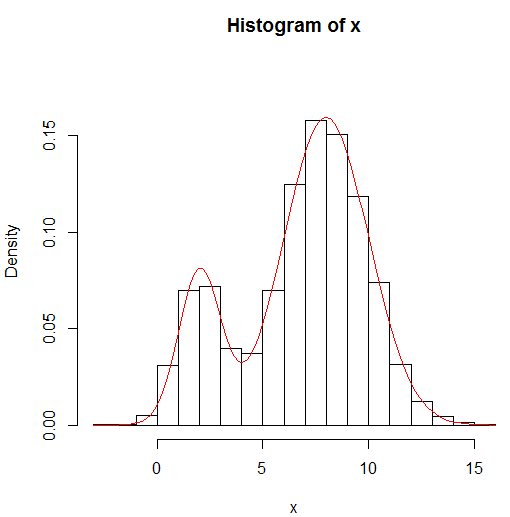
\includegraphics[width=5.5cm]{histr}
			%\caption{Histograma de frecuencias}
		\end{minipage}
	\end{figure}

Vemos que el histograma de los valores simulados se ajusta bien a la curva de densidad de probabilidad de la distribución objetivo.
\newpage

	\begin{figure}[h]
	\hspace*{0.9cm}\begin{minipage}{10.3cm}
		{\setstretch{0.8}
			\begin{lstlisting}[style=myRstyle, caption={Verificación mediante gráfico de cuantiles / MN.}]
# 1. Calcular el cuantil de la distribucion teorica al
#  que pertenece cada valor simulado.
q_t <- p*pnorm(x,u[1],sd[1])+(1-p)*pnorm(x,u[2],sd[2])

# 2. Usar los cuantiles teoricos para extraer el valor
#  simulado correspondiente.
x_q <- quantile(x,q_t)

# 3. Comparar cada valor en su cuantil teorico contra
#  el valor hallado para ese cuantil en la simulacion.
plot(x,x_q)
			\end{lstlisting}
		}			
	\end{minipage}
	\begin{minipage}{6cm}
		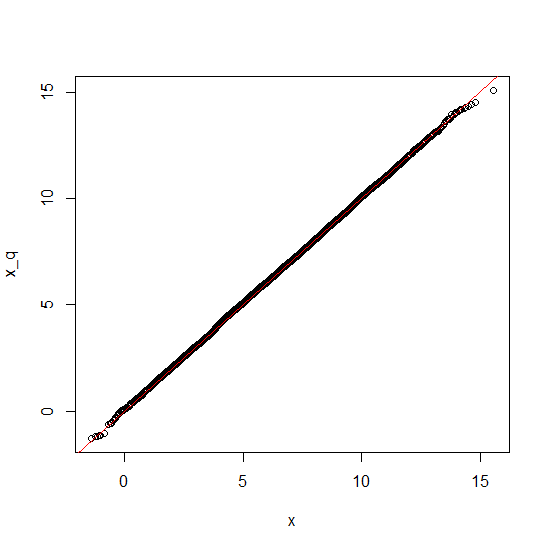
\includegraphics[width=5.5cm]{qu}
		%\caption{Histograma de frecuencias}
	\end{minipage}
\end{figure}

La gráfica de cuantiles muestra una línea casi perfecta, lo cual significa que el valor simulado y el valor teórico en cada cuantil tienen gran cercanía y, por lo tanto, nuestra simulación reproduce adecuadamente la distribución objetivo.

	\end{sol}

\item[d)] Presente los pasos que debe seguir el algoritmo de Metropolis-Hastings considerando como distribución generadora de candidatos una distribución normal centrada en el punto anterior. Implemente en R el algoritmo propuesto. Simule 10 000 valores de una $\text{MN}(2, 8, 1, 4, 0.2)$ y verifique mediante gráficos de cadenas, histograma con función de densidad y cuantiles que el método propuesto funciona correctamente.

\begin{sol} $ $
	
		{\setstretch{0.8}
	\begin{lstlisting}[style=myRstyle, caption={Algoritmo de Metropolis-Hastings.}]
n <- 10000

# Valor inicial basado en la media de la distribucion objetivo
s <- c(p*u[1]+(1-p)*u[2],
numeric(n))

# Recomendacion de Gelman para la varianza de distribucion generadora
sdq <- (p*(sd[1]**2 + u[1]**2)+
(1-p)*(sd[2]**2 + u[2]**2)-
(p*u[1]+(1-p)*u[2])**2)*(2.4**2)

# Definimos funciones objetivo y candidato
d_obj <- function(x){p*dnorm(x,u[1],sd[1])+(1-p)*dnorm(x,u[2],sd[2])}
d_can <- function(x,uc){dnorm(x,uc,sdq)}

# Definimos funcion alpha
alpha <- function(x,y,f,q){
min(1,f(y)*q(x,y)/(f(x)*q(y,x)))
}

# Bucle central del algoritmo
for(i in 1:(length(s)-1)){

# Obtener un valor de la distribucion generadora, condicionado a valor previo.
candidato <- rnorm(1,s[i],sdq)

# Aplicar criterio de aceptacion
if(runif(1)<=alpha(s[i],candidato,d_obj,d_can)){
# Si cumple con criterio, incorporar candidato a la secuencia de valores simulados.
s[i+1] <- candidato
} else {
# Si no cumple con criterio, el valor previo pasa a la siguiente posicion de la secuencia.
s[i+1] <- s[i]
}
}
	\end{lstlisting}
}			
	\begin{figure}[h]
		
	\hspace*{0.9cm}\begin{minipage}{7.3cm}
		{\setstretch{0.8}
			\begin{lstlisting}[style=myRstyle, caption={Revisión del gráfico de cadena / MN.}]
ts.plot(s)
# Distribucion parece estable
# desde el inicio, no haria falta
# retirar observaciones.

			\end{lstlisting}
		}			
	\end{minipage}
	\begin{minipage}{6cm}
		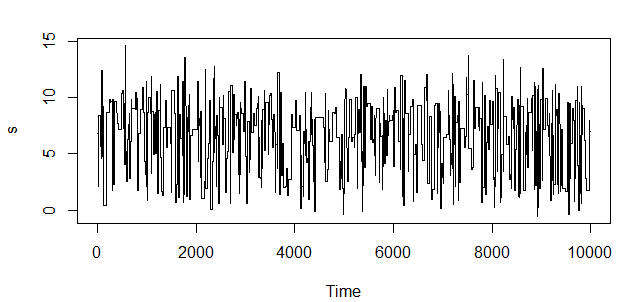
\includegraphics[width=8.5cm]{cad}
		%\caption{Histograma de frecuencias}
	\end{minipage}
\end{figure}

\begin{figure}[h]
	\hspace*{0.9cm}\begin{minipage}{10.3cm}
		{\setstretch{0.8}
			\begin{lstlisting}[style=myRstyle, caption={Verificación mediante histograma / MN.}]
hist(s,probability = TRUE,ylim=c(0,0.18),breaks=25)
curve(p*dnorm(l,u[1],sd[1])+(1-p)*dnorm(l,u[2],sd[2]),
	add = TRUE, xname = "l",col="red")			
			\end{lstlisting}
		}			
	\end{minipage}
	\begin{minipage}{6cm}
		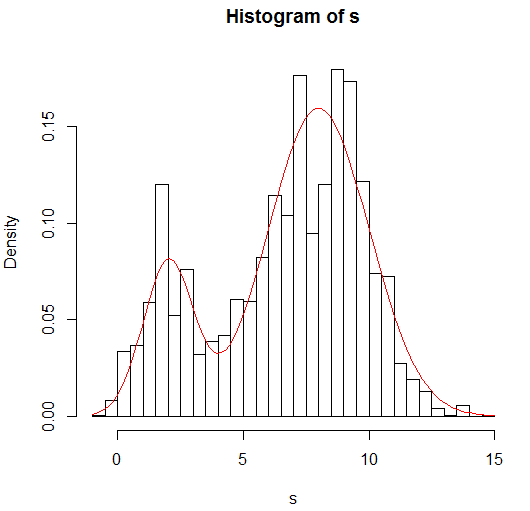
\includegraphics[width=5.5cm]{hist2}
		%\caption{Histograma de frecuencias}
	\end{minipage}
\end{figure}
\begin{figure}[h]
	\hspace*{0.9cm}\begin{minipage}{10.5cm}
		{\setstretch{0.8}
			\begin{lstlisting}[style=myRstyle, caption={Verificación mediante gráfica de cuantiles / MN.}]
# 1. Calcular el cuantil de la distribucion teorica al
#  que pertenece cada valor simulado.
q_t <- p*pnorm(s,u[1],sd[1])+(1-p)*pnorm(s,u[2],sd[2])

# 2. Usar los cuantiles teoricos para extraer el valor
#  simulado correspondiente.
s_q <- quantile(s,q_t)

# 3. Comparar cada valor en su cuantil teorico contra
#  el valor hallado para ese cuantil en la simulacion.
plot(s,s_q)
			\end{lstlisting}
		}			
	\end{minipage}
	\begin{minipage}{6cm}
		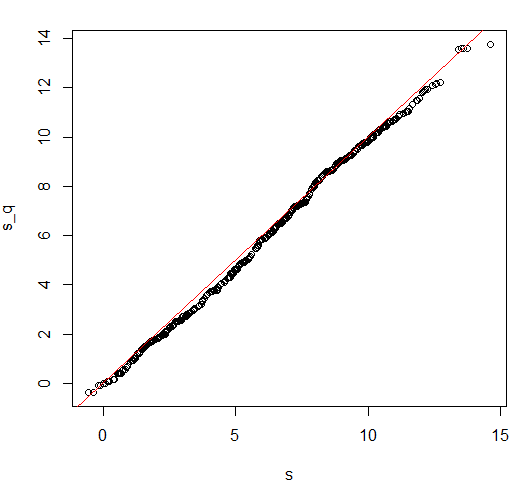
\includegraphics[width=5cm]{qu2}
		%\caption{Histograma de frecuencias}
	\end{minipage}
\end{figure}

Vemos que los valores simulados por Metropolis-Hastings tienen cierta cercanía con la curva teórica en el histograma y se mantienen cercanos a la diagonal en la gráfica de cuantiles, pero en general su ajuste no es tan bueno como el método anterior.
\end{sol}

\end{itemize}
\section*{Ejercicio 2}
Una variable aleatoria definida en toda la recta, tiene distribución normal asimétrica (Azzalini, 1985)
con parámetro de asimetría $\lambda$ si su función de densidad es dada por la siguiente expresión:
$$f_X(x)=2\phi(x)\Phi(\lambda x),\;x\in\mathbb{R}.$$
donde $\phi(\cdot)$ es la 
función de densidad y $\Phi(\cdot)$ es la función de distribución acumulada de una distribución normal estándar y $\lambda\in\mathbb{R}$. Se utiliza la notación $X\sim \text{SN}(\lambda)$.
\begin{itemize}
	\item[a)] Pruebe que una distribución normal estándar puede ser considerada como distribución generadora
	de candidatos en el algoritmo de aceptación y rechazo.
	\begin{sol}
		La implementación del método de aceptación y rechazo para la simulación de $f_X(x)$ toma una función $g_X(x)$, llamada generadora , la cual es fácil de simular y con la que debe cumplirse lo siguiente:
		\begin{eqnarray}
		\dfrac{f_X(x)}{g_X(x)}&\leq &c \;,\;\;\forall x\in\mathbb{R}.
		\end{eqnarray}
		para una constante $c$.\\
		Veamos lo siguiente:
		\begin{eqnarray}
		\dfrac{f_X(x)}{\phi(x)} &=& \dfrac{2\phi(x)\Phi(\lambda x)}{\phi(x)}\nonumber\\
		&=& 2\Phi(\lambda x)\nonumber\\
		&=& 2\int_{-\infty}^{\lambda x}\phi(t)dt\nonumber\\
		&\leq& 2\underbrace{\int_{-\infty}^{\infty}\phi(t)dt}_{=1}\nonumber\\
		&=&2.
		\end{eqnarray}
		Tenemos que $\dfrac{f_X(x)}{\phi(x)}\leq 2$, por lo que $\phi(x)$, además de ser fácil de simular, puede ser considerada como función generadora dado que cumple (9).
	\end{sol}
\newpage
	\item[b)] Presente los pasos que debe seguir el algoritmo de aceptación y rechazo considerando como distribución generadora de candidatos una distribución normal estándar. Implemente en R el algoritmo
	propuesto. Simule $10000$ valores de una $SN(8)$ y 
	verifique mediante gráficos de histograma con
	función de densidad y cuantiles que el método propuesto funciona correctamente.
	\begin{solution}
		La función a simular es la siguiente:
		\begin{eqnarray}
		f_X(x)=2\phi(x)\Phi(8x),\;x\in\mathbb{R}.
		\end{eqnarray}
		Los pasos que se deberían seguir en el algoritmo de aceptación y rechazo serían los siguientes:
		\begin{enumerate}
			\item[1)] Generamos $y\sim N(0,1)$.
			\item[2)] Generamos $u\sim U(0,1)$.
			\item[3)] Si $u\leq \dfrac{f_X(x)}{2\phi(x)} = \Phi(8x)\Rightarrow x=y$. Caso contrario ir al paso 1.
		\end{enumerate}
	A continuación, se presenta un gráfico de la función a simular y la función generadora
	
	\begin{figure}[h]
	\hspace*{0.9cm}\begin{minipage}{10.3cm}
		{\setstretch{0.8}
			\begin{lstlisting}[style=myRstyle, caption={Distribución de interés y distribución normal estándar / SN.}]
curve(2*dnorm(x,0,1)*pnorm(8*x,0,1),0,3,col=1,lwd=2,ylim=c(0,1.5),
xla="x",
ylab="Densidad",
main="Distribucion SN con propuesta normal estandar")
curve(2*dnorm(x,0,1),col=2,lwd=2,add=T)
legend(1.5,1.5,c("f(y)","cg(y)"),col=c(1,2),lty=1,lwd=2,cex=1.2)
			\end{lstlisting}
		}			
	\end{minipage}
	\begin{minipage}{6cm}
		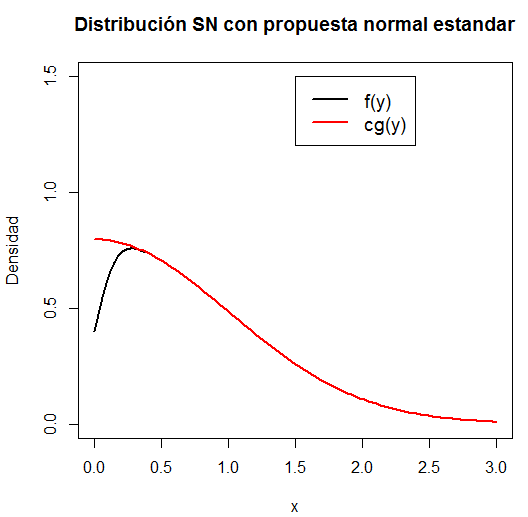
\includegraphics[width=5.5cm]{a1}
		%\caption{Histograma de frecuencias}
	\end{minipage}

\end{figure}
		{\setstretch{0.8}
	\begin{lstlisting}[style=myRstyle, caption={Algoritmo de aceptación y rechazo.}]
M<-10000
x<-numeric(M)

for(h in 1:M){
  cond<-0
  while(cond==0){
    y<-rnorm(1) # Generar un candidato
    u<-runif(1) # Generar u ~ U(0,1)
    if(u <= pnorm(8*y,0,1)){ 
      # Aceptar el candidato
      x[h]<-y
      cond<-1
    }	
  }
}
	\end{lstlisting}
}
	\begin{figure}[h]
	\hspace*{0.9cm}\begin{minipage}{9.8cm}
		{\setstretch{0.8}
			\begin{lstlisting}[style=myRstyle, caption={Verificación mediante histograma / SN.}]
hist(x,probability = TRUE,ylim=c(0,1),breaks=25)
curve(2*dnorm(x,0,1)*pnorm(8*x,0,1),add = TRUE,col="red")
			\end{lstlisting}
		}			
	\end{minipage}
	\begin{minipage}{2cm}
		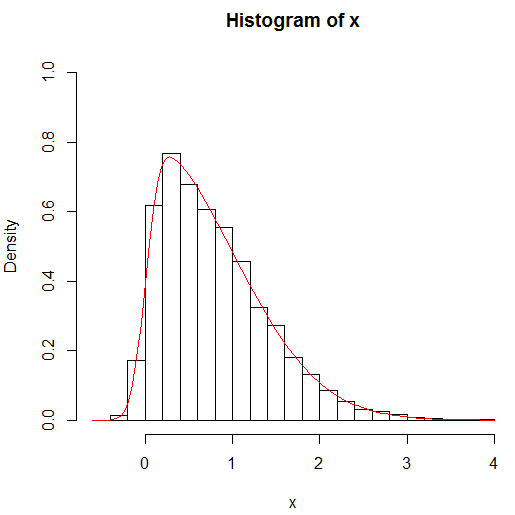
\includegraphics[width=5.5cm]{a2}
		%\caption{Histograma de frecuencias}
	\end{minipage}
\end{figure}
\newpage
	\begin{figure}[h]
	\hspace*{0.9cm}\begin{minipage}{10.3cm}
		{\setstretch{0.8}
			\begin{lstlisting}[style=myRstyle, caption={Verificación mediante gráfica de cuantiles / SN.}]
library(sn)

#Cuantiles muestrales
p=((1:100)-0.5)/100
qm=quantile(x,p)

#Cuantiles poblacionales
qs=qsn(p,alpha = 8)

plot(qm,qs)
abline(0,1,col="red")
			\end{lstlisting}
		}			
	\end{minipage}
	\begin{minipage}{6cm}
		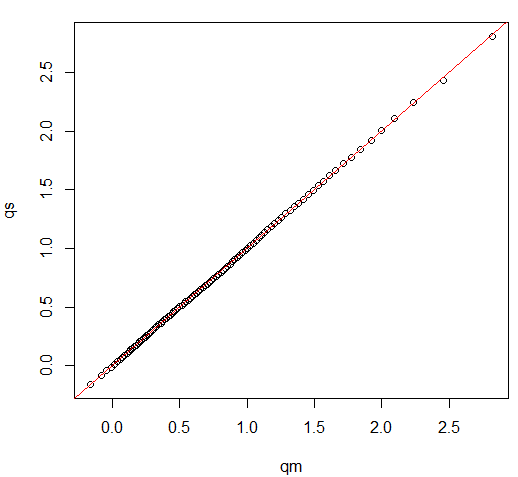
\includegraphics[width=5cm]{a3}
		%\caption{Histograma de frecuencias}
	\end{minipage}
\end{figure}
Se observa, según el histograma, que efectivamente nuestros datos se ajustan correctamente usando una simulación con el método de aceptación y rechazo implementándose como función generadora a la función de densidad normal estandar, $g_X(x)=\phi(x)$.\\
Además, una segunda verificación, mediante un gráfico de cuantiles, nos indica la alta correspondencia entre los datos teóricos y los simulados, corroborando de nuevo la correcta simulación.
	\end{solution}
\end{itemize}

\newpage
\section*{Ejercicio 3}
Una variable aleatoria $X$ definida en toda la recta, tiene distribución logística potencia con parámetro de asimetría $\alpha$ si su función de densidad es dada por la siguiente expresión:
$$f_X(x)=\alpha l(x)L(x)^{\alpha-1},\;x\in\mathbb{R}.$$
donde $l(x)=\dfrac{e^x}{(1+e^x)^2}$ es la función densidad y $L(x)=\dfrac{e^x}{1+e^x}$ es la función de distribución acumulada de una distribución logística estándar, y $\alpha>0$. Se utiliza la notación $X\sim \text{PL}(\alpha)$.
\begin{itemize}
	\item[a)] Encuentre la distribución acumulada de una PL$(\alpha)$.
	\begin{sol}
		Resolviendo $f_X(x)$:
		\begin{eqnarray}
		f_X(x)&=&\alpha l(x)L(x)^{\alpha-1} = \alpha\dfrac{e^x}{(1+e^x)^2}\left(\dfrac{e^x}{1+e^x}\right)^{\alpha-1}=\alpha e^{-x}(1+e^{-x})^{-\alpha-1}.
		\end{eqnarray}
		Derivando $L(x)$ tenemos lo siguiente:
		\begin{eqnarray}
		\dfrac{d(L(x))}{dx}=\dfrac{d\left(\dfrac{e^x}{1+e^x}\right)}{dx}=\dfrac{e^x}{(1+e^x)^2}=l(x)&\Rightarrow&d(L(x))=l(x)dx.
		\end{eqnarray}
		Determinemos ahora $F_X(x)$, la distribución acumulada de $f_X(x)$:
		\begin{eqnarray}
		F_X(x)&=&\int_{-\infty}^{x}f_X(t)dt\nonumber\\
		&=&\int_{-\infty}^{x}\alpha l(t)L(t)^{\alpha-1}dt\nonumber\\
		&=&\int_{-\infty}^{x}\alpha L(t)^{\alpha-1}l(t)dt\nonumber\\
		&\stackrel{\mbox{por }(13)}{=}&\int_{-\infty}^{x}\alpha L(t)^{\alpha-1}d(L(t))\nonumber\\
		&=&L(t)^{\alpha}\big[^{x}_{-\infty}\nonumber\\
		&=&L(x)^{\alpha} -\lim\limits_{t\rightarrow -\infty}L(t)^{\alpha}\nonumber\\
		&=&L(x)^{\alpha} -\lim\limits_{t\rightarrow -\infty}\left(\dfrac{e^t}{1+e^t}\right)^{\alpha}\nonumber\\
		&=&L(x)^{\alpha} -\left(\underbrace{\lim\limits_{t\rightarrow -\infty}\dfrac{e^t}{1+e^t}}_{=0}\right)^{\alpha}\nonumber\\
		&=&L(x)^{\alpha}\nonumber\\
		&=&\left(\dfrac{e^x}{1+e^x}\right)^{\alpha}\;\;,\;\forall x\in\mathbb{R}.
		\end{eqnarray}
	\end{sol}
\item[b)] 	Presente los pasos que debe seguir el algoritmo de transformada inversa. Implemente en R el algoritmo propuesto. Simule 10000 valores de una PL(0.5) y verifique mediante gráficos de histograma y cuantiles que el método propuesto funciona correctamente.
\begin{sol}
	Para usar el método de la transformada inversa, se debe hallar $X=F^{-1}(U)$. De esta manera:
	\begin{eqnarray}
	u = F_X(x)=\left(\dfrac{e^x}{1+e^x}\right)^{\alpha}=(1+e^{-x})^{-\alpha}&\Leftrightarrow& u^{-1/\alpha}=1+e^{-x}\nonumber\\
	&\Leftrightarrow& e^{-x}=u^{-1/\alpha}-1\nonumber\\
	&\Leftrightarrow& -x=\ln\left(u^{-1/\alpha}-1\right)\nonumber\\
	&\Rightarrow& F_X^{-1}(u)=x=\ln\left(\dfrac{1}{u^{-1/\alpha}-1}\right)
	\end{eqnarray}
	\begin{figure}[h]
		\hspace*{0.9cm}\begin{minipage}{10cm}
			{\setstretch{0.8}
				\begin{lstlisting}[style=myRstyle, caption={Verificación mediante histograma / PL.}]
u = runif(10000)
a = 0.5
x = log(1/(u^(-1/a)-1))
fx = function(x){a*exp(-x)*(1+exp(-x))^(-a-1)}

#Grafico de Histograma
par(mfrow=c(1,2))
hist(x,probability = TRUE,xlab="Valores simulados",ylab="Densidad",main="Histograma de los valores simulados")
curve(fx,col=2,lwd=2,add=TRUE)
				\end{lstlisting}
			}			
		\end{minipage}
		\begin{minipage}{6cm}
			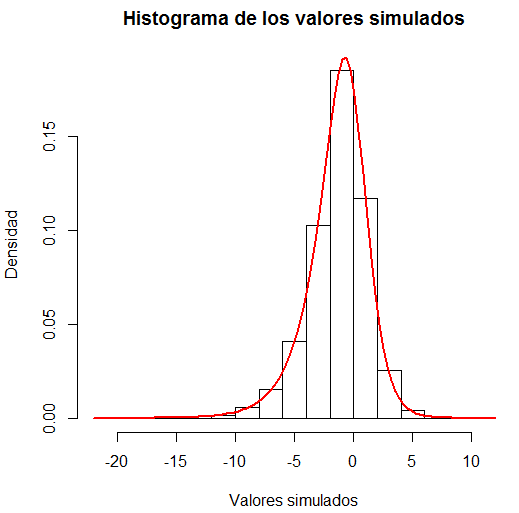
\includegraphics[width=6cm]{hist3}
			%\caption{Histograma de frecuencias}
		\end{minipage}
	\end{figure}
\begin{figure}[h]
	\hspace*{0.9cm}\begin{minipage}{10cm}
		{\setstretch{0.8}
			\begin{lstlisting}[style=myRstyle, caption={Verificación mediante gráfica de cuantiles / PL.}]
p = ((1:100)-0.5)/100

#Calculando los cuantiles muestrales
qm = quantile(x,p)

#Calculando los cuantiles poblacionales
qp = log(1/(p^(-1/a)-1))

plot(qm,qp,pch=16,lwd=2,col=4,main=paste("Grafico de cuantiles"),xlab="Cuantiles muestrales",ylab="Cuantiles teoricos")
abline(0,1,col="red")
			\end{lstlisting}
		}			
	\end{minipage}
	\begin{minipage}{6cm}
		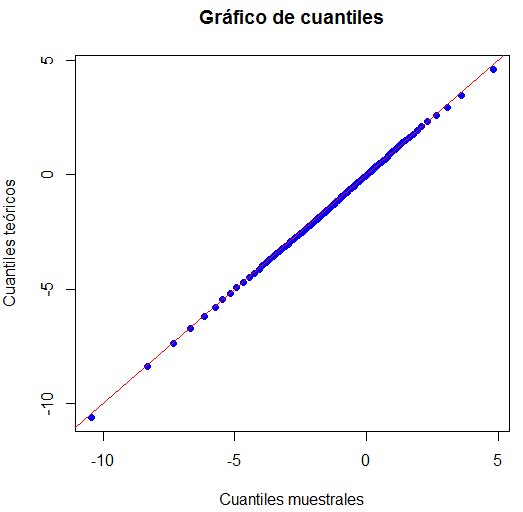
\includegraphics[width=5.8cm]{qu3}
		%\caption{Histograma de frecuencias}
	\end{minipage}
\end{figure}

Para verificar si nuestros datos simulados son correctos, se grafica un histograma con los datos generados por el método de la transformada inversa. Ahora, superponiendo la curva de la distribución logística potencia en el histograma, notamos que los datos se ajustan, por lo que se puede afirmar que la simulación de los datos es apropiada. Asimismo, en el gráfico de cuantiles se aprecia similitud entre los datos simulados y los datos teóricos.

\end{sol}
\end{itemize}

\section*{Ejercicio 4}
Sea $X$ una variable aleatoria con distribución de Gumbel, entonces su función de densidad de probabilidad (f.d.p.) y su función de distribución acumulada (f.d.a.) es dada por
$$f(x)=e^{-x}e^{-e^{-x}}\;\mbox{ y }F(x)=e^{-e^{-x}},\;x\in\mathbb{R}.$$
Una posible generalización es la distribución Gumbel potencia cuya f.d.p. y f.d.a son dadas por
$$f(x)=\alpha e^{-x}\left[e^{-e^{-x}}\right]^{\alpha}\;\mbox{ y }F(x)=\left[e^{-e^{-x}}\right]^{\alpha},\;x\in\mathbb{R},\;\alpha>0.$$
Otra posibilidad es la distribución Gumbel potencia recíproca cuya f.d.p. y f.d.a son dadas por
$$g(x)=\alpha e^{x}\left[e^{-e^{x}}\right]^{\alpha}\;\mbox{ y }G(x)=1-\left[e^{-e^{x}}\right]^{\alpha},\;x\in\mathbb{R},\;\alpha>0.$$
\begin{itemize}
	\item[a)] Verificar si las f.d.p. de las distribuciones: Gumbel potencia y Gumbel potencia reciproca son log-concava.
	\begin{sol} Sabemos para que una función $h(x)$ sea log-cóncava, debe cumplirse lo siguiente:
		\begin{eqnarray}
		\dfrac{d^2(\log(h(x)))}{dx^2}<0,\;x\in\mathbb{R}.
		\end{eqnarray}
		\begin{itemize}
			\item Verificación sobre la distribución Gumbel potencia:
			\begin{eqnarray}
			&&f(x)=\alpha e^{-x}\left[e^{-e^{-x}}\right]^{\alpha} = \alpha e^{-x-\alpha e^{-x}}\nonumber\\
			&\Rightarrow& \log(f(x)) = \log(\alpha) -x-\alpha e^{-x}
			\end{eqnarray}
		Veamos que la función descrita en (17) cumple ser log-cóncava,
		\begin{eqnarray}
		\dfrac{d(\log(f(x)))}{dx} &=&-1+\alpha e^{-x}\nonumber\\
		\dfrac{d^2(\log(f(x)))}{dx^2} &=&-\alpha e^{-x} <0\;\;\;\forall x\in\mathbb{R}.
		\end{eqnarray}
		Esto último se debe a que $\alpha>0$ y $e^{-x}>0$ para todo $x\in\mathbb{R}$.
		\item Verificación sobre la distribución Gumbel potencia recíproca:
		\begin{eqnarray}
		&&g(x)=\alpha e^{x}\left[e^{-e^{x}}\right]^{\alpha} = \alpha e^{x-\alpha e^{x}}\nonumber\\
		&\Rightarrow& \log(g(x)) = \log(\alpha) +x-\alpha e^{x}
		\end{eqnarray}
		Veamos que la función descrita en (19) cumple ser log-cóncava,
		\begin{eqnarray}
		\dfrac{d(\log(g(x)))}{dx} &=&1-\alpha e^{x}\nonumber\\
		\dfrac{d^2(\log(g(x)))}{dx^2} &=&-\alpha e^{x} <0\;\;\;\forall x\in\mathbb{R}.
		\end{eqnarray}
		Esto último se debe a que $\alpha>0$ y $e^{x}>0$ para todo $x\in\mathbb{R}$.
		\end{itemize}
	\end{sol}
\newpage
\item[b)] Implemente el método ARS en R. Simule 10,000 valores para cada 
distribución, considere $\alpha=2$.
Realice un gráfico de histograma con la función de densidad y un gráfico de cuantiles.
\begin{sol}$ $
{\setstretch{0.8}
	\begin{lstlisting}[style=myRstyle, caption={Método ARS / Definiciones Iniciales.}]
M<-10000
a<-2
p<-((1:100)-0.5)/100
	\end{lstlisting}
}	

{\bf $\bullet$ Método de ARS en R para la función de distribución de Gumbel:}

{\setstretch{0.8}
	\begin{lstlisting}[style=myRstyle, caption={Algoritmo ARS / GUMBEL.}]
library(ars)

f1<-function(x,mu=0,sigma=1){-x-exp(-x)}
f1prima<-function(x,mu=0,sigma=1){-1+exp(-x)}
y<-ars(10000,f1,f1prima,mu=0,sigma=1)
	\end{lstlisting}
}			
	\begin{figure}[h]
	\hspace*{0.9cm}\begin{minipage}{10cm}
		{\setstretch{0.8}
			\begin{lstlisting}[style=myRstyle, caption={Verificación mediante histograma / GUMBEL.}]
hist(y,prob=T)
curve(exp(-x)*exp(-exp(-x)),col=2,add=T)
			\end{lstlisting}
		}			
	\end{minipage}
	\begin{minipage}{6cm}
		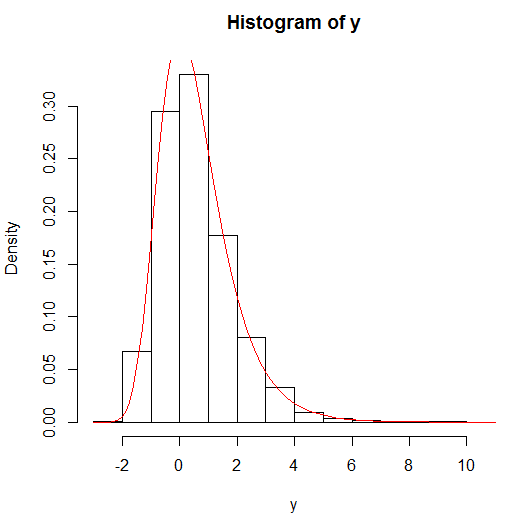
\includegraphics[width=5.5cm]{hist4}
		%\caption{Histograma de frecuencias}
	\end{minipage}
\end{figure}
	\begin{figure}[h]
	\hspace*{0.9cm}\begin{minipage}{10cm}
		{\setstretch{0.8}
			\begin{lstlisting}[style=myRstyle, caption={Verificación mediante gráfica de cuantiles / GUMBEL.}]
library(lattice)

qqmath(y,distribution=function(p){-log(-log(p))})
			\end{lstlisting}
		}			
	\end{minipage}
	\begin{minipage}{6cm}
		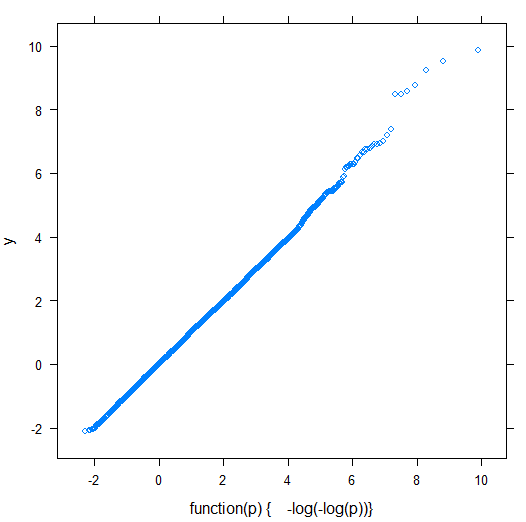
\includegraphics[width=5.6cm]{mi0}
		%\caption{Histograma de frecuencias}
	\end{minipage}
\end{figure}
\newpage
{\bf Método de ARS en R para la función de distribución de Gumbel potencia:}
{\setstretch{0.8}
	\begin{lstlisting}[style=myRstyle, caption={Algoritmo ARS / GUMBEL POTENCIA.}]
library(ars)

f<-function(x,a){log(a)-x-a*exp(-x)}
fprima<-function(x,a){-1+a*exp(-x)}
gp<-ars(M,f,fprima,a=2)
	\end{lstlisting}
}

\begin{figure}[h]
	\hspace*{0.9cm}\begin{minipage}{10cm}
		{\setstretch{0.8}
			\begin{lstlisting}[style=myRstyle, caption={Verificación mediante histograma / GUMBEL POTENCIA.}]
hist(gp,prob=T,xlab="Valores Simulados",ylab="Densidad",main="Histograma de los valores simulados")
fx<-function(x){a*exp(-x)*(exp(-exp(-x)))^a}
curve(fx,col=2,lwd=2,add=T)
			\end{lstlisting}
		}			
	\end{minipage}
	\begin{minipage}{6cm}
		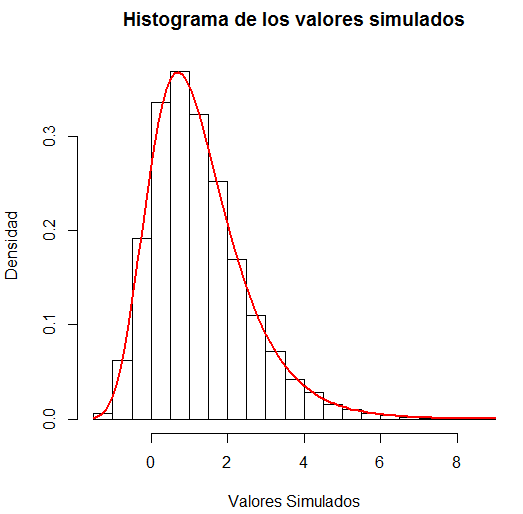
\includegraphics[width=5.5cm]{mi2}
		%\caption{Histograma de frecuencias}
	\end{minipage}
\end{figure}
\begin{figure}[h]
	\hspace*{0.9cm}\begin{minipage}{10cm}
		{\setstretch{0.8}
			\begin{lstlisting}[style=myRstyle, caption={Verificación mediante gráfica de cuantiles / GUMBEL POTENCIA.}]
qqmath(gp,distribution=function(p){log(a)-log(log(1/p))})
			\end{lstlisting}
		}			
	\end{minipage}
	\begin{minipage}{6cm}
		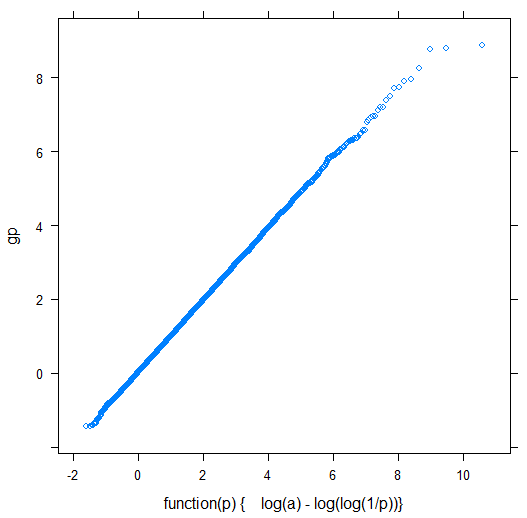
\includegraphics[width=5.5cm]{mi3}
		%\caption{Histograma de frecuencias}
	\end{minipage}
\end{figure}

{\bf Método de ARS en R para la función de distribución de Gumbel potencia recíproca:}
{\setstretch{0.8}
	\begin{lstlisting}[style=myRstyle, caption={Algoritmo ARS / GUMBEL POTENCIA RECÍPROCO.}]
library(ars)
	
g<-function(x,a){log(a)+x-a*exp(x)}
gprima<-function(x,a){1-a*exp(x)}
gpr<-ars(M,g,gprima,a=2)
	\end{lstlisting}
}

\newpage
\begin{figure}[h]
	\hspace*{0.9cm}\begin{minipage}{10cm}
		{\setstretch{0.8}
			\begin{lstlisting}[style=myRstyle, caption={Verificación mediante histograma / GUMBEL POTENCIA RECÍPROCO.}]
hist(gpr,prob=T,xlab="Valores Simulados",ylab="Densidad",main="Histograma de los valores simulados")
gx<-function(x){a*exp(x)*(exp(-exp(x)))^a}
curve(gx,col=2,lwd=2,add=T)
			\end{lstlisting}
		}			
	\end{minipage}
	\begin{minipage}{6cm}
		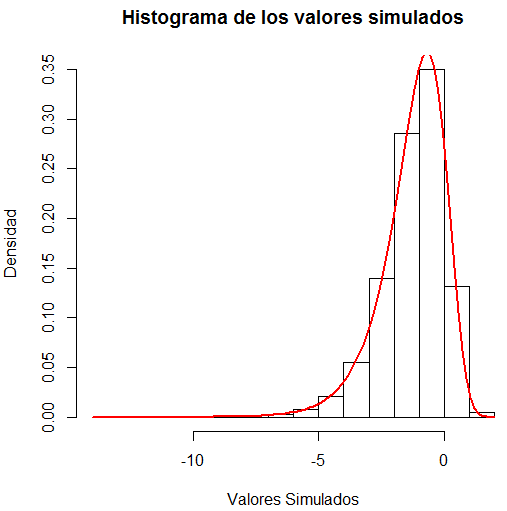
\includegraphics[width=5.5cm]{mi4}
		%\caption{Histograma de frecuencias}
	\end{minipage}
\end{figure}
\begin{figure}[h]
	\hspace*{0.9cm}\begin{minipage}{10cm}
		{\setstretch{0.8}
			\begin{lstlisting}[style=myRstyle, caption={Verificación mediante gráfica de cuantiles / GUMBEL POTENCIA RECÍPROCO.}]
qqmath(gpr,distribution=function(p){-log(a)+log(log(1/(1-p)))})
			\end{lstlisting}
		}			
	\end{minipage}
	\begin{minipage}{6cm}
		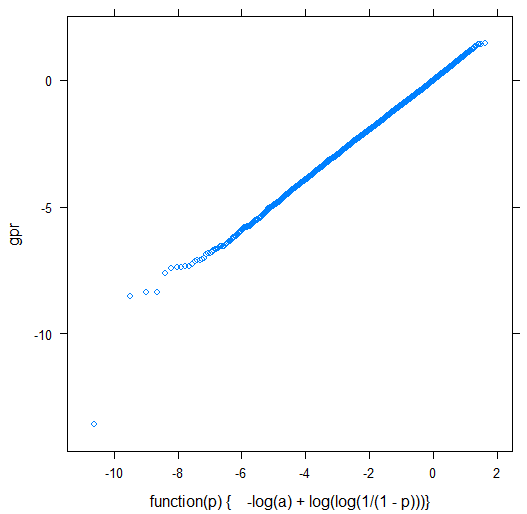
\includegraphics[width=5.5cm]{mi5}
		%\caption{Histograma de frecuencias}
	\end{minipage}
\end{figure}

Se ha podido demostrar que las 3 funciones , f.d.p. de Gumbel, f.d.p. de Gumbel potencia y f.d.p. de Gumbel potencia recíproca, se ha podido generar las muestras de variables aleatorias, dado que cada una ha cumplido dos condiciones:
\begin{itemize}
	\item[i)] Las 3 funciones son continuas y diferenciables en todo su dominio $R_X$. Es diferenciable porque las funciones admiten derivadas en cualquier dirección y puede aproximarse al menos hasta primer orden. Es continua pues para cualquier punto $x=a$ , existe $f(a)$, asimismo también existe el límite de la función en el punto $x=a$ y finalmente $f(a)$ coincide con el límite de la función en el punto.
	\begin{eqnarray}
	&&\exists f(a)\\
	&&\exists\lim\limits_{x\rightarrow a}f(x)\Leftrightarrow \lim\limits_{x\rightarrow a^-}f(x)=\lim\limits_{x\rightarrow a^+}f(x)\\
	&&f(a)=\lim\limits_{x\rightarrow a}f(x)
	\end{eqnarray}
	\item[ii)] La función log-cóncava de cada una cumple que su segunda derivada es menor que CERO, para todo $x\in R_X$.
\end{itemize}
Gracias a que $log f(x)$, $log f(x)$ potencia y $log g(x)$ son funciones cóncavas, estas han podido ser acotadas superiormente por sus tangentes, lo cual ha permitido que se haya podido acercar cada vez más a las  funciones.\\
\newpage
{\bf Gráfico de las 3 funciones}:
\begin{figure}[h]
	\hspace*{0.9cm}\begin{minipage}{9cm}
		{\setstretch{0.8}
			\begin{lstlisting}[style=myRstyle, caption={Gráfico de las 3 funciones / GUMBEL.}]
curve(exp(-x)*exp(-exp(-x)),from=-8, to=8,col=2,add=T)
curve(2*exp(-x)*(exp(-exp(-x)))^2,from=-8, to=8,col=3,add=T)
curve(2*exp(x)*(exp(-exp(x)))^2,from=-8, to=8,col=4,add=T)
			\end{lstlisting}
		}			
	\end{minipage}
	\begin{minipage}{6cm}
		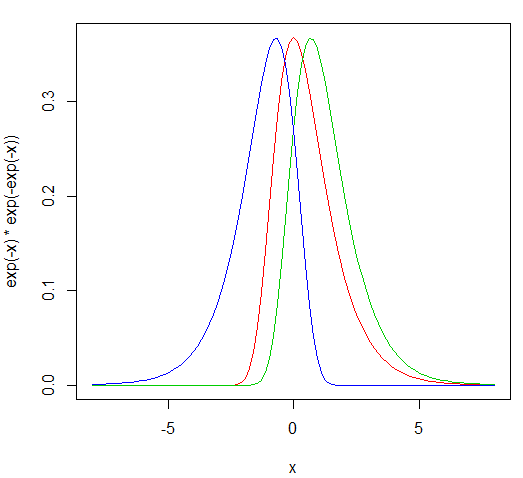
\includegraphics[width=6.6cm]{3di}
		%\caption{Histograma de frecuencias}
	\end{minipage}
\end{figure}
\end{sol}
\end{itemize}
\end{document}